\documentclass[conference]{IEEEtran}
\usepackage{amsmath,amssymb,graphicx,booktabs,url}
\newcommand{\BookSpeedup}{4.87}
\newcommand{\HotMedianRange}{96.1--103.9}
\newcommand{\HotPninetyRange}{140.4--164.8}
\newcommand{\ThroughputRange}{16.08--20.37}

\newcommand{\SpacingMaxRatio}{14}
\newcommand{\SpacingOneMsRatio}{5}
\newcommand{\SpacingHundredRatio}{2.9}
\newcommand{\HostBHotMedianRange}{158.2--161.1}
\newcommand{\HostBHotPninetyRange}{333.9--356.8}
\newcommand{\HostBThroughputRange}{8.47--9.90}
\newcommand{\HostBBookSpeedup}{4.58}
\newcommand{\HostBCpu}{Intel Xeon  @ 2.80GHz}

\title{Spacing Matters: Back-to-Back Replay Understates Tick-to-Trade Latency in a Reproducible C++ Market-Data Pipeline}
\author{\IEEEauthorblockN{Rajvardhan Jadhav}\IEEEauthorblockA{Fox School of Business, Temple University\\Philadelphia, PA, USA}}
\begin{document}\maketitle
\begin{abstract}
Tick-to-trade latency of low-latency trading software is commonly measured by replaying recorded packets back to back. We show on a C++20 pipeline (feed arbitration, order book, market-making decision, risk, order management, order-entry staging) that this practice understates per-tick cost once packets are spaced as they would be on a real feed. Inserting an idle gap \emph{outside} the timed interval, with no cache pollution by the benchmark itself, raises the median no-order tick latency by \SpacingHundredRatio$\times$ at a 100~\textmu s gap and by \SpacingOneMsRatio$\times$ at 1~ms, on a shared cloud VM, using a build whose full-session replay is verified byte-exact against the backtest before any latency is reported. Separate observations from a 60-second live public-feed capture documented in the repository show the same direction. We also report the first timing replication of the artifact on a second host, a matched book-update baseline, and paired synthetic strategy ablations with Holm-corrected inference. Running the pipeline's code path on a shadow instance during the gap recovers only part of the penalty, and the mechanism is not isolated (no hardware counters are available in these VMs), and nothing here measures exchange latency or profitability. The contribution is a measurement-methodology finding plus a fully reproducible artifact.
\end{abstract}
\begin{IEEEkeywords}tick-to-trade latency, benchmarking methodology, order book, reproducibility, C++\end{IEEEkeywords}

\section{Introduction}
Reported tick-to-trade figures for software trading systems are frequently obtained by replaying a captured session as fast as the pipeline will accept it. This keeps caches, branch predictors and prefetchers warm and so yields the best case. A live system receives a market-data packet every few hundred microseconds to tens of milliseconds, during which the same core may execute other code or sit idle. How much the best-case number understates the cost of a tick at realistic spacing is rarely reported together with the artifact needed to check it.

This paper makes three claims, each tied to preserved raw outputs.
\begin{enumerate}
\item \textbf{Spacing effect.} In a pinned, single-thread replay of a byte-verified session, an idle gap before each tick increases measured latency by large factors (Section~\ref{sec:spacing}) without the benchmark evicting its own working set.
\item \textbf{Artifact and replication.} The complete pipeline, tests, experiment drivers and manuscript generator reproduce from one command; hot-cache timings were replicated on a second host (Section~\ref{sec:host}).
\item \textbf{Honest scope.} A matched book-update baseline and paired synthetic strategy ablations are reported with their limits; no profitability, formal-verification or exchange-latency claim is made.
\end{enumerate}
The pipeline design combines familiar techniques; novelty lies in the measurement finding and in the end-to-end evidence chain, not in a new algorithm.

\section{Related Work}
Limit order book structure and dynamics are surveyed in~\cite{gould2013}; stochastic and queue-reactive models are in~\cite{cont2010,huang2015}, and queue position valuation in~\cite{moallemi2017}. Market-making theory under inventory risk is classically treated in~\cite{avellaneda2008}, and latency-driven market design in~\cite{budish2015}. These works concern market models, not software latency measurement, and we use them only to place the synthetic strategy experiments.

On benchmarking methodology, measurement bias from seemingly irrelevant experimental setup was shown in~\cite{mytkowicz2009}; statistically rigorous benchmarking with a bounded number of repetitions in~\cite{kalibera2013}; and reporting practice for scientific benchmarking of parallel systems in~\cite{hoefler2015}. Our spacing experiment is a concrete instance of this concern in a trading-system context.

The phenomenon itself is known to practitioners. Because the order-sending path of a trading system executes rarely, its code and data are often cold when it is needed; the C++ low-latency design literature describes cache warming, for example running the engine on every event but releasing orders only when needed, and reports a large benefit in a cold-versus-warm microbenchmark~\cite{bilokon2023}. That benchmark compares access patterns over a data set rather than sweeping idle time between invocations. Open-source matching engines such as~\cite{jericevich2021} report latency and throughput tests. In the sources we could access, we did not find a controlled sweep of idle time between ticks with a matched back-to-back control for an inspectable end-to-end pipeline; this is a statement about our search, not a priority claim (Section~\ref{sec:limits}).

\section{Pipeline}
An encoded feed packet passes through A/B arbitration, gap detection and snapshot recovery, order-book update, a market-making decision, pre-trade risk, order management and order-entry staging, in one thread run to completion. The book uses flat price levels, pooled intrusive order nodes, a bitmap and an ID table; the 32-byte node size is a compile-time check, not a proof of cache behaviour. A compile target checks selected hot-path headers with exceptions and RTTI disabled. The benchmark excludes NIC reception, kernel networking, TLS, JSON parsing and the exchange. Correctness checks are differential (independent reference book and replay hash), not formal verification.

The strategy combines a spread, an order-book-imbalance lean and an inventory skew with risk limits; its coefficients are engineering choices and no optimal-control claim is made.

\section{Measurement Method}
\textbf{Timed interval.} Each tick is timed with ordered TSC reads around ingest and decide; the p50 timer overhead (about 14--15~ns) is subtracted. Ticks are classified as \emph{order} (at least one order frame staged) or \emph{no-order} (tick-to-decision). The histogram stores bin counts and tick calibration; quantiles use nearest rank $\lceil qn\rceil$ (a predecessor bug used $\lfloor qn\rfloor$).

\textbf{Verification gate.} Before any latency is printed the production pipeline must emit the backtest session's exact wire bytes (hash match). A failed match aborts the run. The gapped passes replay a prefix of the same session through the same code path, so they are not themselves re-hashed.

\textbf{Hosts.} Host~A: shared AMD EPYC 9V74 VM, four-core quota, GCC~14. Host~B (\HostBCpu): shared VM with two vCPUs, GCC~13.3. Neither has hardware performance counters, CPU isolation or a fixed frequency. Both are cloud VMs of the same provider class, so the replication tests software and compiler variation and not hardware diversity.

\textbf{Spacing control.} For each gap $g$ a spin loop of $g$ before every tick, outside the timed interval, is compared with a gap-0 pass over the same first $N$ inputs, so the only difference is idle time between ticks. For large $g$, $N$ is reduced so a pass takes about two seconds ($N=40{,}000$ for $g\le20$~\textmu s, down to $300$ at 10~ms). The spin executes no memory traffic, so it does not evict the benchmark's own working set. Ratios are computed per run and the median over five sequential runs is reported.

\section{Spacing Results}\label{sec:spacing}
Table~\ref{tab:spacing} and Fig.~\ref{fig:spacing} give median-of-five results on Host~B (the same code with the shadow-warming option, described below, was added to the benchmark before these runs).
\begin{table}[t]\centering\caption{Median over five runs: no-order tick p50, its ratio to the matched gap-0 control, no-order p50 with shadow warming, and order-tick p50. Source: \texttt{results/spacing/*/benchmark\_*.json}. Few order ticks remain at gaps of 1~ms and above (37 and 12 per run), so those order p50 values are descriptive; the 10~ms row uses only 300 inputs.}\label{tab:spacing}\begin{tabular}{rrrrrr}\hline Gap (µs) & $N$ & No-order p50 (ns) & vs.\ control & Warmed (ns) & Order p50 (ns)\\\hline
1 & 40000 & 98 & 1.0$\times$ & -- & 177\\
5 & 40000 & 105 & 1.1$\times$ & 107 & 234\\
20 & 40000 & 164 & 1.7$\times$ & 188 & 328\\
100 & 20000 & 291 & 2.9$\times$ & 254 & 634\\
1000 & 2000 & 531 & 5.0$\times$ & 394 & 1714\\
10000 & 300 & 2742 & 14.1$\times$ & 1188 & 3291\\
\hline\end{tabular}\end{table}
\begin{figure}[t]\centering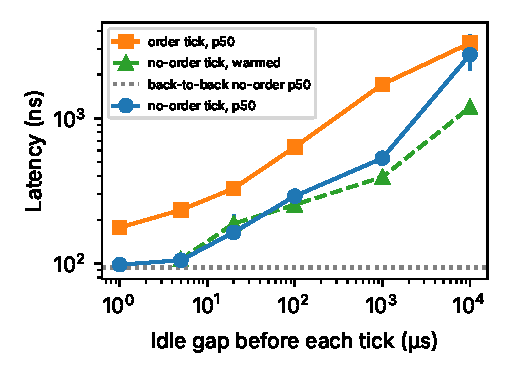
\includegraphics[width=\columnwidth]{figures/spacing.pdf}\caption{Latency versus idle gap (log--log); bars show the min--max of the five-run p50. Dotted line: back-to-back no-order p50.}\label{fig:spacing}\end{figure}
Latency rises monotonically beyond a gap of a few microseconds and is a large multiple of the back-to-back figure by 1~ms. The no-order p99 also rises, from 0.24~\textmu s back to back to about 1.1~\textmu s at 100~\textmu s and 2.0~\textmu s at 1~ms. At the 10~ms gap the five-run ratio ranged from 10$\times$ to 18$\times$, reflecting only 274 no-order samples per run. For scale, a deliberately harsh cold-cache case (a 4~MiB walk before every tick, first 40{,}000 inputs, five runs) gave no-order p50 of 708--720~ns and order p50 of 1.42--1.55~\textmu s; the idle-gap result cannot be attributed to the benchmark's own eviction because the spin touches no memory.

\textbf{Partial mitigation by code-path warming.} Following the cache-warming practice noted in Section~II, a second \emph{shadow} pipeline instance, fed its own copy of the session, processes five inputs in the last 3~\textmu s of each gap, so the same code runs without touching the live book's data or sending anything. The ``Warmed'' column of Table~\ref{tab:spacing} shows the no-order p50. Warming recovers part of the penalty only at long gaps (1~ms: from 531 to 394~ns; 10~ms: from 2.74 to 1.19~\textmu s) and none at 20 and 100~\textmu s. Code-path warming alone therefore does not remove the effect; the remaining penalty is consistent with decay of the live book's data in cache or with predictor state specific to that data, but this was not isolated.

\textbf{What is not shown.} We have not isolated the cause. State decay in caches, branch predictors or TLBs, descheduling or noisy neighbours on the shared VM, and frequency or idle-state effects are all consistent with the data. The p50 is robust to rare descheduling, which argues against pure scheduler noise, but a bare-metal replication with performance counters is required to attribute the effect.

\section{Live-Feed Observations}\label{sec:live}
The repository documents a live paper-mode session on a public BTC-USD level-2 feed (60--90~s captures, \texttt{docs/LIVE\_PAPER.md}). Replaying the same 60-second capture with different gaps between messages gave per-message p50 of 18.4~\textmu s back to back and 63.5~\textmu s at the recorded spacing (about 57~ms), roughly 3.5$\times$; spinning instead of sleeping did not change this. That workload includes JSON parsing and conversion, which dominate (the pipeline itself is about 1.3~\textmu s per packet), so absolute values are not comparable to Table~\ref{tab:spacing}. We report it because the direction agrees. \textbf{These live observations were taken by the repository author on a different VM (Xeon 2.1~GHz, two vCPUs), the capture is not in the repository, and they were not reproduced by this paper's pipeline.} They should be treated as corroborating, not as evidence.

\section{Cross-Host Replication and Book Baseline}\label{sec:host}
Hot-cache order-tick p50 ranged \HotMedianRange~ns on Host~A and \HostBHotMedianRange~ns on Host~B; p99 \HotPninetyRange~ns versus \HostBHotPninetyRange~ns; sustained throughput \ThroughputRange\ versus \HostBThroughputRange\ million inputs/s. Absolute figures therefore differ across hosts by roughly 1.6$\times$ at p50 and 2$\times$ in throughput, even though both are shared cloud VMs, so they are host-specific. They are also best-case, back-to-back numbers and should be read with Section~\ref{sec:spacing}.

An offline operation benchmark compares the flat book with an independent \texttt{std::map}/\texttt{std::list} reference over five seeded tapes of 200{,}000 timed mixed operations, requiring identical return values and state digests. The median speed ratio was \BookSpeedup\ on Host~A and \HostBBookSpeedup\ on Host~B, so this relative result was stable across hosts. This is a book-update baseline, not a comparison against a tuned third-party engine.

\section{Synthetic Strategy Ablations}
The queue-aware synthetic backtester stages orders through the production gateway and OMS. The generator includes informed flow that imbalance reveals, so removing the imbalance lean tests whether the signal is used, not whether alpha exists. The primary run uses 16 markets (seeds 1000--1015) and a confirmation run seeds 5000--5015; paired differences use Student-$t$ intervals, exact sign tests and Holm correction~\cite{holm1979} over a four-comparison family. Fills are not independent replicates.
\begin{table}[t]\centering\caption{Primary paired synthetic PnL differences versus the base. CI is Student-$t$ for mean difference; $p$ is Holm-adjusted exact sign-test probability. Source: \texttt{paired\_statistics.csv}.}\resizebox{\columnwidth}{!}{\begin{tabular}{lrrr}\hline Variant & Paired gain & 95\% CI & Holm $p$\\\hline
noalpha & -16.78 & [-17.53,-16.03] & 0.0001221\\
wide & -17.27 & [-18.18,-16.36] & 0.0001221\\
noskew & 7.45 & [1.80,13.09] & 0.2101\\
strongskew & -4.82 & [-5.27,-4.38] & 0.0001221\\
\hline\end{tabular}}\end{table}
Removing imbalance substantially reduces simulated PnL, consistent with the generator's design; removing inventory skew raises mean PnL while holding larger positions. Regime, fee, queue, latency-sweep and held-out selection results are preserved in the artifact. Delay in the latency sweep applies to each of three hops. None of this establishes a profitable live strategy.

\section{Limitations and Threats to Validity}\label{sec:limits}
\textbf{Mechanism.} The spacing effect is measured, not explained; the warming test narrows but does not settle the cause. \textbf{Hosts.} Two shared cloud VMs, five sequential runs each, no isolation, no performance counters; no bare-metal result. \textbf{Spin gap.} A spin loop is one model of idle time; real feeds interleave other code and interrupts, and the tiny spin loop could itself perturb predictor or frequency state. \textbf{Small $N$ at large gaps.} Order-tick statistics at gaps above 100~\textmu s rest on few samples. \textbf{Synthetic data.} The recorded session and strategy results are generated; the live observations are not reproduced here. \textbf{Baselines.} The map/list reference is deliberately simple. \textbf{Literature.} A systematic search of the low-latency systems literature for prior controlled spacing measurements has not been completed, and several references were verified only against bibliographic records and not full texts. No claim of priority is made. \textbf{Scope.} Nothing measures network, NIC, kernel or exchange latency, real fills, market impact or profitability.

\section{Reproduction}
With CMake, Ninja, GCC, Python dependencies pinned in \texttt{research/requirements-lock.txt} and TeX Live, \texttt{bash research/reproduce.sh} builds, tests, runs the experiments, regenerates figures and tables and compiles this PDF. The spacing study is \texttt{research/run\_spacing\_study.py} followed by \texttt{research/analyze\_spacing.py}. No exchange credentials or orders are used.

\section*{Acknowledgment}
\textbf{AI disclosure (author to confirm before submission).} The C++ source, tests, experiment scripts and portions of this manuscript's text, tables and figures were produced with the assistance of Anthropic's Claude (including Claude Code), under the author's direction. The author is responsible for the content. [Author to state, per IEEE policy, which sections used AI-generated content and at what level.]

\bibliographystyle{ieeetr}\bibliography{references}
\end{document}
